\subsection*{Report 4}

In figure \ref{figure:2_2}, the previously used train signal is reshaped into segments of 20ms, on which the DFT is applied to each segment. Enlarging the segment size will give a better resolution on the frequency axis, but lower on the time axis. The DFT gives the frequency content of a the whole sample, but does not distinguishing when this frequency was present. By splinting up the sample, we can see the frequency content change in steps of 20ms through time. However, while smaller segment size gives better time resolution, it results in worse frequency resolution, with the opposite also being true. This is due to the number of samples in the window decreasing for smaller audio segments, meaning the resulting frequency domain graph also has less defined frequencies it displays.

	\begin{figure}[H] 
		\centering
		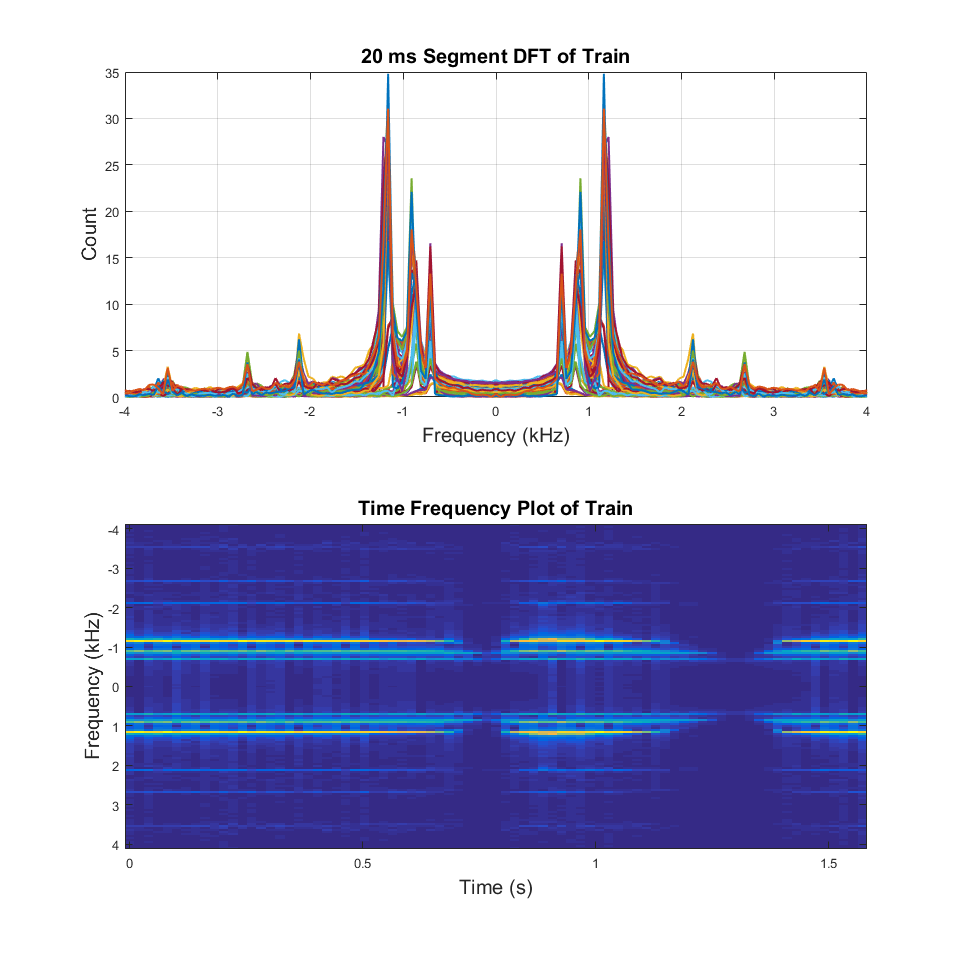
\includegraphics[width=\textwidth]{2.2.png}
		\caption{Train - Segmented FFT \& Time Frequency Plot}
		\label{figure:2_2}
	\end{figure}
	
	